\subsection{TCE Transit Fits}
\label{s:fits}
The \Kepler\ Pipeline fits each TCE with a \citet{Mandel2002} transit model using \citet{Claret2000} limb darkening parameters. After the transit searches were performed for the observed, injected, scrambled, and inverted TCEs, we discovered that the transit fit portion of DV had an error that caused the impact parameter for each fit to be biased towards large values, causing the planet radii to be systematically too large (for further information see \citealt{Christiansen2017} and \citealt{Coughlin2017a}). Since a consistent set of reliable transit fits are required for all TCEs, we refit the transits.  The same DV transit fitting code was corrected for the bug and seeded with the \Kepler{} identification number, period, epoch, and MES of the original detection. These ``supplemental'' DV fits do not have the same impact parameter bias as the original.  Sometimes the DV fitter fails to converge and in these cases we were not able to obtain a supplemental DV transit fit, causing us to fall back on the original DV fit. Also, at times the epoch wanders too far from the original detection; in these cases we do not consider it to be a successful fit and again fall back on the original fit.

The creation of this KOI catalog depends on four different transit fits: 1) the original DV transit fits, 2) the trapezoidal fits performed on the ALT \citet{Garcia2010} detrended light curves, 3) the supplemental DV transit fits, and 4) the MCMC fits (see \S\ref{s:mcmc}).  Because the bug in the transit fits was only discovered after all of the metrics for the Robovetter were run, the original DV and trapezoidal fits were used to disposition all of the sets of TCEs. These are the same fits that are available for the \opstce{s} in the DR25 TCE table at the Exoplanet Archive. Most Robovetter metrics are agnostic to the parameters of the fit, and so the supplemental DV fits would only change a few of the Robovetter decisions. While the Robovetter itself runs in a few minutes, several of the metrics that feed the Robovetter (see Appendix \ref{s:metrics}) require weeks to compute, so we chose not to update the metrics in order to achieve this minimal improvement. And for all sets of TCEs, the original DV fits are listed in the Robovetter input files\footnote{Robovetter input files have the format kplr\_dr25\_XXX\_robovetter\_input.tar.gz and can be found in the Robovetter github repository, \url{https://github.com/nasa/kepler-robovetter}}. The supplemental fits are used to understand the completeness and reliability of the catalog as a function of fitted parameters (such as planet radii or insolation flux). For all sets of TCEs, the supplemental DV fits are available as part of the Robovetter results tables linked from the TCE documentation page\footnote{The Robovetter results files are linked under the Q1-Q17 DR25 Information on the page \url{https://exoplanetarchive.ipac.caltech.edu/docs/Kepler\_TCE\_docs.html}} for the \opstce{s} and from the simulated data page\footnote{\url{https://exoplanetarchive.ipac.caltech.edu/docs/KeplerSimulated.html}} \citep[see][]{Christiansen2017,Coughlin2017a} for the injected, inverted, and scrambled TCEs. The MCMC fits are only provided for the KOI population and are available in the DR25 KOI table\footnote{\url{https://exoplanetarchive.ipac.caltech.edu/cgi-bin/TblView/nph-tblView?app=ExoTbls\&config=q1\_q17\_dr25\_koi}} at the Exoplanet Archive. The MCMC fits have no consistent offset from the supplemental DV fits.  To show this, we plot the planet radii derived from the two types of fits for the planet candidates in DR25 and show the distribution of fractional change in planet radii; see Figure~\ref{f:mcmcsupp}. The median value of the fractional change is 0.7\% with a standard deviation of 18\%. While individual systems disagree, there is no offset in planet radii between the two populations. The supplemental DV fitted radii and MCMC fitted radii agree within 1-sigma of the combined error bar (i.e., the square-root of the sum of the squared errors) for 78\% of the KOIs and 93.4\% of PCs (only 1.8\% of PC's radii differ by more than 3-sigma).  The differences are caused by discrepancies in the detrending and because the MCMC fits include a non-linear ephemeris in its model when appropriate (i.e., to account for transit-timing variations).

\begin{figure}[htb]
\centering
\begin{tabular}{c}
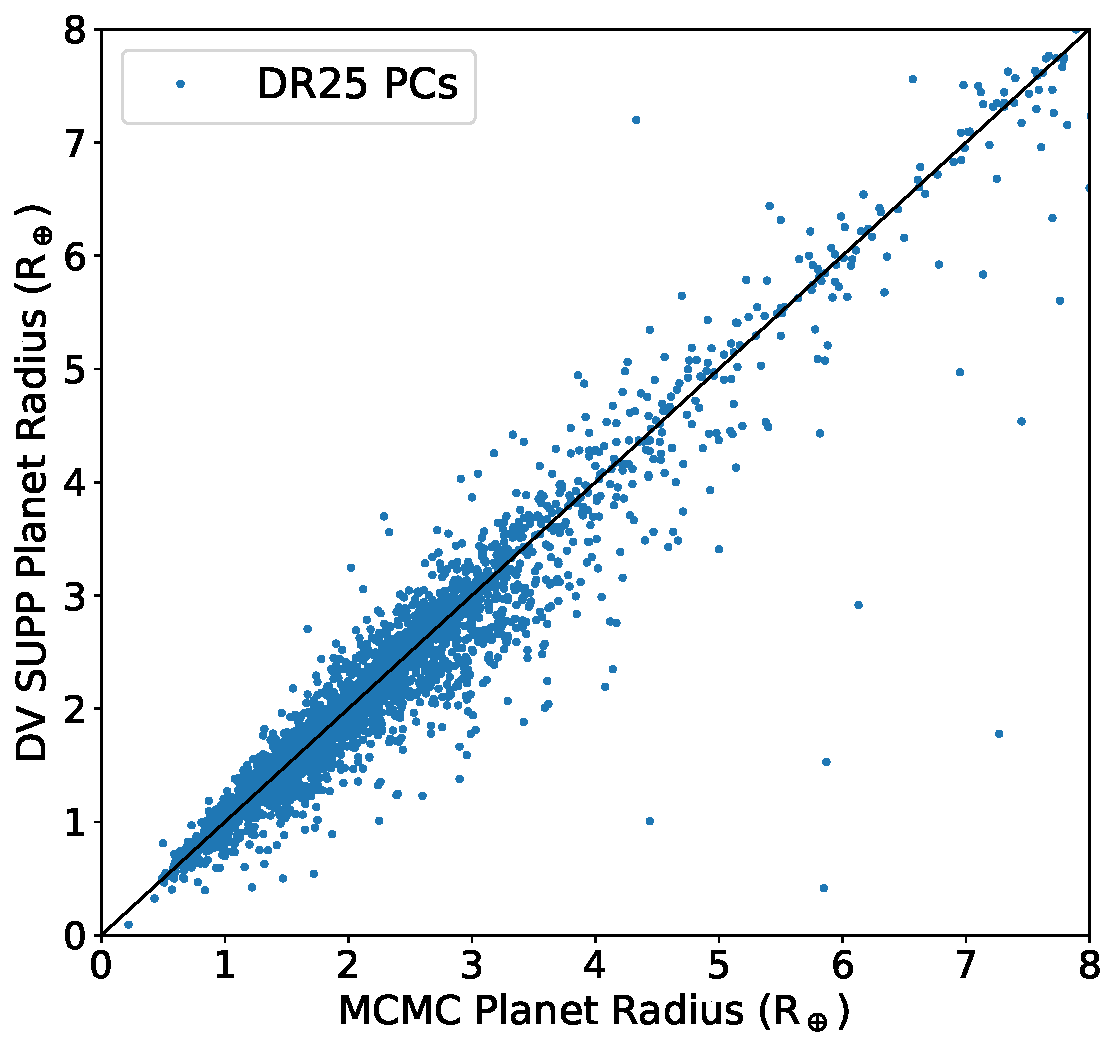
\includegraphics[width=\linewidth]{f3-top.pdf} \\[2em]
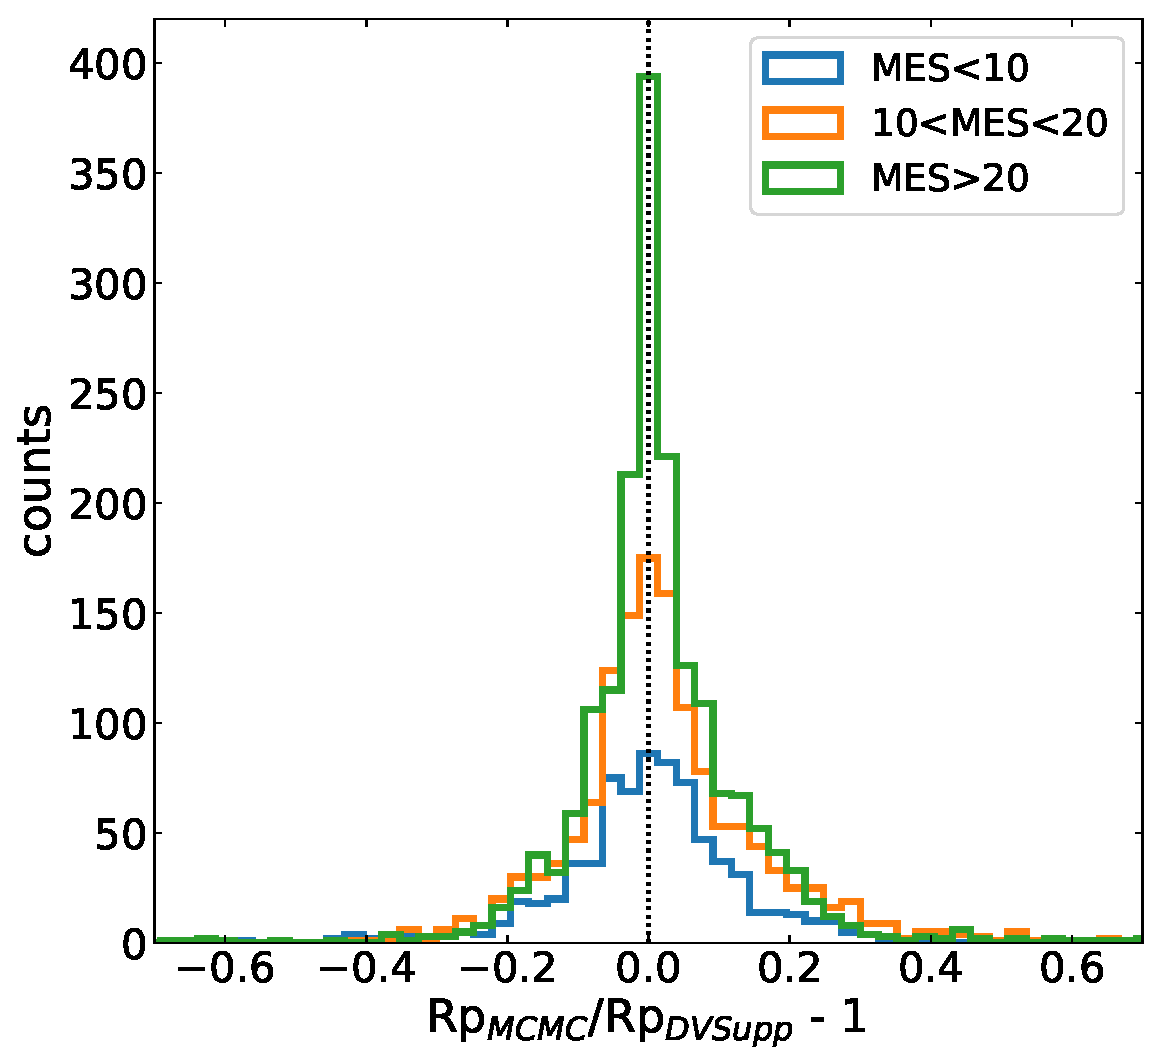
\includegraphics[width=\linewidth]{f3-bottom.pdf}
\end{tabular}
\caption{Top: Comparison of the DR25 PCs fitted planet radii measured by the MCMC fits and the DV supplemental fits. The 1:1 line is drawn in black. Bottom: Histogram of the difference between the MCMC fits and the DV fits for the planet candidates in different MES bins. While individual objects have different fitted values, as a group the planet radii from the two fits agree. }
\label{f:mcmcsupp}
\end{figure}


\subsection{Stellar Catalog}
\label{s:stars}
Some of the derived parameters from transit fits (e.g., planetary radii and insolation flux) of the TCEs and KOIs rely critically on the accuracy of the stellar properties (e.g., radii, mass, and temperature). For all transit fits used to create this catalog we use the DR25 Q1--Q17 stellar table provided by \citet{Mathur2017ApJS}, which are based on conditioning published atmospheric parameters on a grid of Dartmouth isochrones \citep{Dotter2008}. The best-available observational data for each star is used to determine the stellar parameters; e.g., asteroseismic or high-resolution spectroscopic data, when available, is used instead of broad-band photometric measurements. Typical uncertainties in this stellar catalog are $\approx$27\% in radius, $\approx$17\% in mass, and $\approx$51\% in density, which is somewhat smaller than previous catalogs.

After completion of the DR25 catalog an error was discovered: the metallicities of 780 KOIs were assigned a fixed erroneous value ([Fe/H] = 0.15 dex). These targets can be identified by selecting those that have the metallicity provenance column set to "SPE90". Since radii are fairly insensitive to metallicity and the average metallicity of \Kepler stars is close to solar, the impact of this error on stellar radii is typically less than 10\% and does not significantly change the conclusions in this paper. Corrected stellar properties for these stars will be provided in an upcoming erratum to \citet{Mathur2017ApJS}. The KOI catalog vetting and fits rely exclusively on the original DR25 stellar catalog information. Because the stellar parameters will continue to be updated (with data from missions such as \emph{Gaia}, \citealt{gaia1,gaia2}) we perform our vetting and analysis independent of stellar properties where possible, and provide the fitted information relative to the stellar properties in the KOI table.  A notable exception is the limb darkening values needed for the transit fits. However, limb-darkening coefficients are fairly insensitive to the most uncertain stellar parameters in the stellar properties catalog (e.g., surface gravity; \citealt{Claret2000}).
